%xelatex
%shell-escape для minted
\documentclass[a4paper, 12pt, oneside]{extarticle}
\input{$UNI/.templates/settings/preamble.tex}
\input{$UNI/.templates/settings/font_styles.tex}
\input{$UNI/.templates/settings/minted_settings.tex}
\addbibresource{~/Documents/uni/bibliography.bib}

\usepackage[explicit]{titlesec}
% \usepackage[svgnames]{xcolor}

\renewcommand\Variant{
$$
\begin{cases}
	a + b + c + d + e &= 6 \\
-0.3 a + 2.3 b - 0.4 c - 0.4 d - 0.2 e &= 1.2  \\
-0.8 a - 0.6 b + 1.5 c - 0.8 d - 0.6 e &= -1.56  \\
-0.3 a - 0.9 b - 0.4 c + 2.1 d &= 0.6  \\
-0.7 a - 0.4 b - 0.7 c - 0.4 d + 1.7 e &= -0.6
\end{cases}
$$
	}
% \newcommand\Date{DAY.MONTH.\the\year}
\newcommand\Type{\Lab} % \Lab \Pract \RGR
\Work{num}
% \newcommand\Number{NUMBER}
\newcommand\Topic{
	Чисельне розв’язування \\
системи лінійних алгебраїчних \\
рівнянь (№ 4)
}

\usepackage[breakable]{tcolorbox}

\usepackage{blindtext}

\titleformat{\section}
[display]
{\color{black}\normalfont\bfseries}
{}
{0pt}
{\begin{tcolorbox}[arc=0mm, colback=blue!10!white, boxrule=0.2mm, beforeafter skip=0pt, boxsep=0mm]{ #1}\end{tcolorbox}}

\titleformat{\subsection}
[display]
{\color{black}\normalfont\bfseries}
{}
{0pt}
{\begin{tcolorbox}[arc=0mm, colback=blue!10!white, boxrule=0.2mm, beforeafter skip=0pt, boxsep=0mm]{ #1}\end{tcolorbox}}

\titlespacing*{\section}{0pt}{0ex}{-4ex}
\titlespacing*{\subsection}{0pt}{0ex}{-4ex}

\usepackage{multirow}
\usepackage{makecell}
\usepackage{tabularx}

% \setlength{\textfloatsep}{12pt}
\newcommand\tcobx[1]{
\begin{tcolorbox}[breakable, arc=0mm, colback=white, boxrule=0.2mm, beforeafter skip=0pt]
	#1
\end{tcolorbox}
}

\begin{document}
\Margins

\Margins
%\begin{wrapfigure}[3]{l}{.27\textwidth}
%\includegraphics[width=.28\textwidth]{$UNI/.templates/lpnu_logo.png}
%\end{wrapfigure}

%\noindent\textbf{Прізвище:} \Lname \\
%\noindent\textbf{Ім'я:} \Fname \\
%\noindent\textbf{Група:} \Group \\
%\noindent\textbf{Варіант:} \Variant \\
%\noindent\textbf{Дата захисту:} \Date \\
%\\
%\noindent\textbf{Кафедра:} \Department \\
%\noindent\textbf{Дисципліна:} \Discipline \\
%\noindent\textbf{Перевірив:} \Instructor \\

%%\medskip\bigskip

%\begin{center}
%	\textbf{ЗВІТ}		\\
%	до \Type~\No\Number	\\
%	на тему ``\Topic''	\\
%\end{center}

% \begin{table}
%   \begin{tabularx}{\textwidth}{|c|X|X|}
%     \hline
%     % Image & Content & Additional Info \\
%     % \hline
% 	  \multirow{3}{*}{\includegraphics[width=4cm]{$UNI/.templates/lpnu_logo.png}}
% 	  & \textbf{ЗВО:}
% 	  Національний університет ``Львівська Політехніка''.
% 	  & \textbf{Тема:}
% 	  \Topic
% 	  \\
% 	  & \textbf{Навчальний рік:}
% 	  2023/2024
% 	  & \textbf{Інститут}
% 	  комп'ютерних наук та інформаційних технологій
% 	  \\
% 	  & \textbf{Семестр:}
% 	  осінній
% 	  & \textbf{Група:}
% 	  \Group
% 	  \\
% 	  & \textbf{Навчальна дисципліна:}
% 	  \Discipline
% 	  & \textbf{Студент:}
% 	  Мілюхін Олександр
% 	  \\
% 	  & \textbf{Кафедра}
% 	  систем автоматизованого проектування
% 	  &
% 	  \\
% 	  & \textbf{Викладач:}
% 	  Чумакевич В. В.
% 	  &
% 	  \\
%     \hline
%   \end{tabularx}
% \end{table}

\setlength{\textfloatsep}{-16pt}
% \setlength{\intextsep}{0pt}

\begin{table}
	\begin{tabular}{|l|l|p{6cm}|}
    \hline
    % Image & Content & Additional Info \\
    % \hline
	  \makecell[l]{
	  \includegraphics[width=3.37cm]{$UNI/.templates/lpnu_logo.png}
  }
	  & \makecell[l]{
	  \textbf{ЗВО:}
	  Національний університет \\ ``Львівська Політехніка''.
	  \\
	  \textbf{Навчальний рік:}
	  2023/2024
	  \\
	  \textbf{Семестр:}
	  осінній
	  \\
	  \textbf{Навчальна дисципліна:} \\
	  \Discipline
	  \\
	  \textbf{Кафедра}
	  систем автоматизованого \\ проектування
	  \\
	  \textbf{Викладач:}
	  Чумакевич В. В.
}
	  & \makecell [l] {
	  \textbf{Тема:}
	  \Topic
	  \\
          \textbf{Інститут}
	  комп'ютерних наук та \\ інформаційних технологій
	  \\
	  \textbf{Група:}
	  \Group
	  \\
	  \textbf{Студент:}
	  Мілюхін Олександр
  }
  \\
    \hline
  \end{tabular}
\end{table}
\section{Мета роботи}

% \begin{table}
%   \begin{tabularx}{\textwidth}{|p{6cm}|c|c|}
% 	  \hline
%     \multirow{3}{*}{\includegraphics[width=6cm]{$UNI/.templates/lpnu_logo.png}}
% 	  & ЗВО: Національний університет ``Львівська Політехніка''
% 	  & Additional Info 1 \\
%     & Content 2 & Additional Info 2 \\
%     & Content 3 & Additional Info 3 \\
% 	  \hline
%   \end{tabularx}
% \end{table}

% \begin{table}
%   \begin{tabular}{|c|c|c|}
%     \hline
%     \multirow{3}{*}{\includegraphics[width=3cm]{$UNI/.templates/lpnu_logo.png}} & \makecell{Content 1 \\ Content 2 \\ Content 3} & \makecell{Additional Info 1 \\ Additional Info 2 \\ Additional Info 3} \\
%     \hline
%   \end{tabular}
% \end{table}

% мета
\tcobx{
	Розв’язати систему лінійних алгебраїчних рівнянь метод Гауса і методом Гауса — Зейделя.
}

\section*{Завдання}
\tcobx{
1. Згідно із варіантом, одержати систему лінійних рівнянь.

2. Перетворити систему лінійних алгебраїчних рівнянь у векторно-матричну форму A x = B.

3. Скласти програму, яка визначає розв’язок цієї системи на основі метода Гауса та на основі
метода Гауса — Зейделя.

4. Запустити програму на виконання та одержати результат через консоль.

5. Звести результатами обчислення до таблиць, побудувати графік зміни поточного наближення
розв’язку залежно від номера ітерації.
}

\section*{Дані згідно з варіантом}

\tcobx{
	\Variant
}

\section*{ Матриця $A$ та вектор-стовпець $B$ }

\tcobx{
$$
A = \begin{bmatrix}
1 & 1 & 1 & 1 & 1  \\
-0.3 & 2.3 &- 0.4 &- 0.4 &- 0.2  \\
-0.8 &- 0.6 & 1.5 &- 0.8 &- 0.6  \\
-0.3 &- 0.9 &- 0.4 & 2.1 & 0 \\
-0.7 &- 0.4 &- 0.7 &- 0.4 & 1.7
\end{bmatrix},\,
B = \begin{bmatrix}
6 \\
1.2  \\
-1.56  \\
0.6  \\
-0.6
\end{bmatrix}
$$
}

\section*{ Код програми}

\tcobx {
	\inputminted{c++}{sle.cpp}
}

\section*{ Вивід}

\tcobx {
	\small
	\verbatiminput{out}
	\normalsize
}

% \end{document}
\section*{ Результати обчислення}

\subsection*{ Результат обчислення методом Гауса }

\tcobx {
$$
X = \begin{bmatrix}
1.2 \\
1.2  \\
1.2  \\
1.2  \\
1.2
\end{bmatrix}
$$
}

\subsection*{ Таблиця з результатами обчислення для методу Гауса-Зейделя}

\tcobx {
\csvautolongtable{table.csv}
}

\subsection*{ Графік зміни поточного наближення розв’язку для методу Гауса – Зейделя}

\tcobx {
	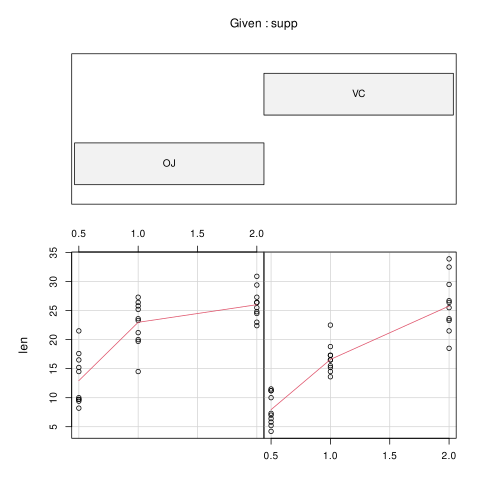
\includegraphics[width=\textwidth]{plot}
}

\section*{ Висновок}

\tcobx {
	Я склав програму мовою C++ для обчислення СЛАР
	метом Гауса та Гауса-Зейделя.
	для системи

	\Variant
	розв'язки:
	\begin{itemize}
		\item $ X = \{ 1.2 , 1.2  , 1.2  , 1.2  , 1.2 \} $ --- точний методом Гауса
		\item $ X = \{ 1.19e+00,1.20e+00,1.20e+00,1.20e+00,1.20e+00 \} $ --- наближений Гауса-Зейделя
	\end{itemize}
}

\end{document}

/* std::vector <std::vector <double> > A = { */
/* 	{1,	1,	1,	1,	1}, */
/* 	{-0.5,	1.8,	-0.9,	-0.1,	-0.8}, */
/* 	{0,	-0.3,	2.5,	-0.6,	-0.4}, */
/* 	{0,	-0.9,	-0.8,	1.4,	0}, */
/* 	{0,	-0.5,	0,	-0.5,	1.5} */
/* }; */
/* std::vector <double> B = {15,	-1.5,	3.6,	-0.9,	1.5}; */

\section*{ <++> }

\subsection*{ <++> }

\tcobx{
	<++>
}

\subsection*{ <++> }

\tcobx {
	<++>
}
